\documentclass{article}

\usepackage{graphicx}
\usepackage{listings}
\usepackage{indentfirst}
\usepackage[a4paper, total={6in, 8in}]{geometry}
\usepackage{hyperref}
\usepackage{fancyhdr}
\usepackage{xepersian}

\settextfont{B Nazanin}
\setlatintextfont{Times New Roman}

\begin{document}


%title page%
\begin{titlepage}
	\begin{center}
		\textbf{ \Huge{به نام خدا}}
	
		\vspace{0.2cm}		
		
\includegraphics[width=0.4\textwidth]{sharif.png}\\
		\vspace{0.2cm}
		\textbf{ \Huge{آزمایش شماره 7}}\\
		\vspace{0.25cm}
		\textbf{ \Large{آز معماری - دکتر سربازی آزاد}}
		\vspace{0.2cm}
		
		
		\large \textbf{دانشکده مهندسی کامپیوتر}\\\vspace{0.1cm}
		\large   دانشگاه صنعتی شریف\\\vspace{0.2cm}
		\large   ﻧﯿﻢ‌سال اول ۰۰-۰۱ \\\vspace{0.10cm}
		\large{\href{mailto:a.h.hadian@gmail.com}{امیرحسین هادیان - ۹۷۱۰۲۶۰۹}}\\
		\large{\href{mailto:mofayezi.m@gmail.com}{محمدرضا مفیضی - ۹۸۱۰۶۰۵۹}}\\
		\large{\href{mailto:a.hatam008@gmail.com}{علی حاتمی تاجیک - ۹۸۱۰۱۳۸۵}}\\
	\end{center}
\end{titlepage}
%title page%

\newpage

%pages header
\pagestyle{fancy}
\fancyhf{}
\fancyfoot{}
\setlength{\headheight}{59pt}
\cfoot{\thepage}
\lhead{آزمایش شماره 7}
\rhead{
\includegraphics[width=0.1\textwidth]{sharif.png}\\
		دانشکده مهندسی کامپیوتر
}
\chead{آز معماری}
%pages header

\section{هدف}
هدف از انجام این آزمایش افزودن حافظه داده برای نگه‌داشتن داده‌ها (به خاطر محدودیت تعداد رجیستر) و همینطور افزودن دستورات شرطی به مجموعه دستورات را داریم.

\section{طراحی}
در این بخش به (باز)طراحی ماشین می‌پردازیم. این طراحی از دو بخش کلی اعمال تغییرات در آزمایش قبل متناسب با نیاز‌های جدید و همینطور طراحی و پیاده‌سازی بخش‌های جدید نیز مانند مموری، بافر سه ‌حالته و خط باس داده و همینطور واحد کنترل نیز باید طراحی شوند. شکل \ref{fig:main} نمایانگر مدار نهایی است.

\begin{figure}
	\centering
	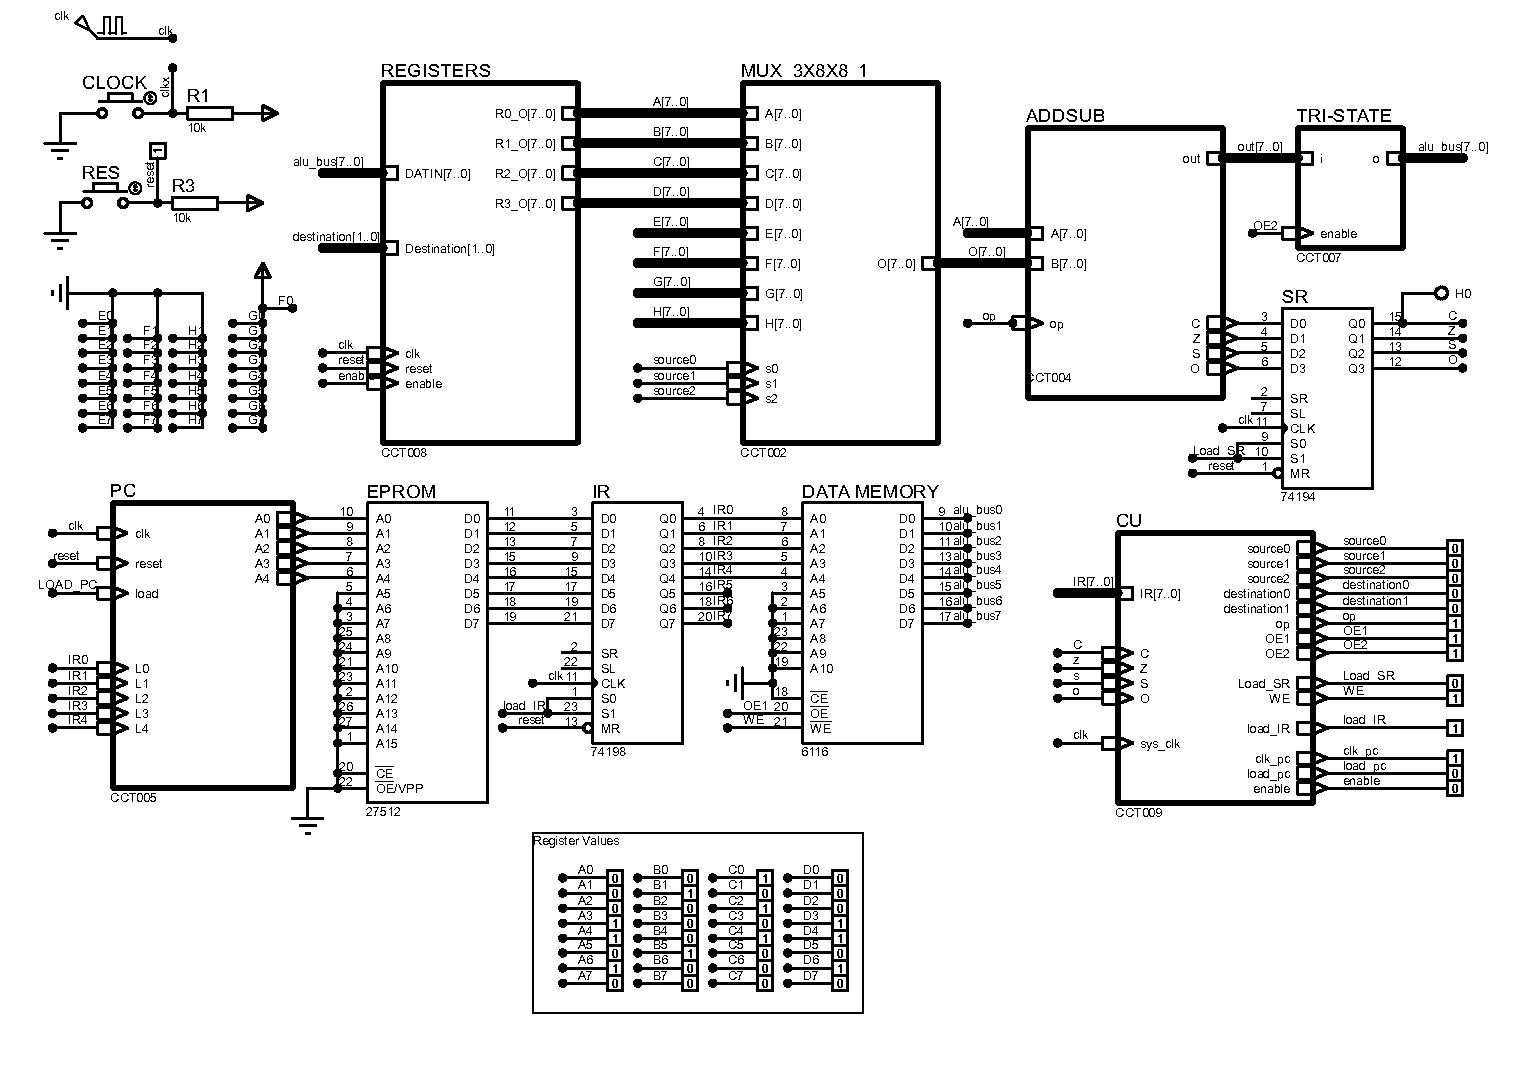
\includegraphics[scale=0.5,page=1]{./graphics/graphics}
	\caption{مدار اصلی}
	\label{fig:main}
\end{figure}
\subsection{تغییرات در مدل آزمایش قبل}
در این بخش به تغییراتی که در آزمایش قبل ایجاد شده است می پردازیم.

\subsubsection{تغییرات \lr{PC}}
در این آزمایش شمارنده برنامه نیاز به قابلیت لود دارد که در شمارنده قبلی وجود نداشت. برای همین از دو تراشه 4516 (شمارنده چهاربیتی) استفاده شده است و از خروجی یکی به عنوان کلاک دیگری استفاده شده است تا یک شمارنده ۵ بیتی بدست بیاید. این تراشه‌ها دارای قابلیت لود هستند. شکل شمارنده برنامه جدید در تصویر \ref{fig:pc} آمده است.

\begin{figure}
	\centering
	\includegraphics[scale=0.6,page=5]{./graphics/graphics}
	\caption{\lr{Program Counter}}
	\label{fig:pc}
\end{figure}

\subsubsection{تغییرات \lr{ALU}}
جمع کننده و تفریق کننده نیاز به سیگنالهای خروجی بیت نقلی، صفر، سرریز و علامت است که به خاطر اینکه برای تشخیص سرریز نیاز به کری ورودی و خروجی بیت آخر داریم جمع کننده‌های فعلی کارا نخواهند بود و به همین خاطر از هشت تمام جمع کننده استفاده شده است تا به این بیت ها دسترسی داشته باشیم. حاصل کار در شکل \ref{fig:as} آمده است.

\begin{figure}
	\centering
	\includegraphics[scale=0.5,page=3]{./graphics/graphics}
	\caption{جمع/تفریق کننده}
	\label{fig:as}
\end{figure}

\subsection{طراحی‌های جدید}
\subsubsection{بافر سه حالته}
برای خواندن و نوشتن روی مموری و تداخل نداشتن داده ها نیاز به یک باس داده هستیم جلوگیری از ورود داده‌های جمع/تفریق کننده به وسیله چند بافر سه حالته بدست می‌آید. شکل \ref{fig:tri} نشان‌دهنده این بخش است.

\begin{figure}
	\centering
	\includegraphics[scale=0.5,page=6]{./graphics/graphics}
	\caption{بافر سه حالته}
	\label{fig:tri}
\end{figure}

\subsubsection{\lr{RAM}}
از یک تراشه 6116 (\lr{SRAM}) برای نگه‌داری داده‌های بینابینی استفاده شده است. سیگنال های نوشتن/خواندن فعال بودن آن توسط واحد کنترل نوشته می‌شود و آدرس ورودی آن از مقدار ثبات دستور می‌آید.


\subsubsection{واحد کنترل}
در واحد کنترل برای تولید سیگنال های کنترلی با توجه به اینکه دستور از چه نوعی است (نوشتن/خواندن، دستورات منطقی/حسابی و یا دستورات پرش)‌ تولید شده‌اند. همینطور کنترل ثبات پرچم ها نیز توسط این بخش تولید می‌شود که تنها در مواقع مناسب تغییر کنند. ساختار ساده این بخش در شکل \ref{fig:CU} آمده است.


\begin{figure}
	\centering
	\includegraphics[scale=0.5,page=7]{./graphics/graphics}
	\caption{واحد کنترل}
	\label{fig:CU}
\end{figure}

\section{تست}
برای تست ماشین ساخته شده از دو برنامه گفته شده استفاده می‌کنیم.

\subsection{جمع فیبوناچی}
کد برنامه به صورت زیر است:
\begin{latin}
\begin{lstlisting}
			sub 	R0,R0		00100000 -> 20
			add		R2,0		00010100 -> 14
			add 	R3,1		00011101 -> 1D
			add		R1,1		00001101 -> 0D
			add		R0,1		00000101 -> 05
			add		R0,1		00000101 -> 05
			add		R0,R0		00000000 -> 00
			store	counter		01100001 -> 61
	loop:	sub		R0,R0		00100000 -> 20
			add		R0,R2		00000010 -> 02
			add		R0,R1		00000001 -> 01
			add		R1,R1		00001001 -> 09
			add		R2,0		00010100 -> 14
			add		R3,R3		00011011 -> 1B
			sub		R0,R0		00100000 -> 20
			add 	R0,R1		00000001 -> 01
			add		R3,R3		00011011 -> 1B
			load	counter		01000001 -> 41
			sub		R0,1		00100101 -> 25
			jz		end			10010110 -> 96
			store	counter		01100001 -> 61
			jmp		loop		11101000 -> E8
	end:	sub		R0,R0		00100000 -> 20
			add		R0,R3		00000011 -> 03
			store	sum			01100000 -> 60
	endd:	jmp		endd		11111001 -> F9
	
	
--
sum 0
counter 1
\end{lstlisting}
\end{latin}

که با توجه به برنامه نتیجه مورد نظر در ثبات سه و صفر موجود است. نتیجه تست در شکل \ref{fig:test1}
آمده است.

\begin{figure}
	\centering
	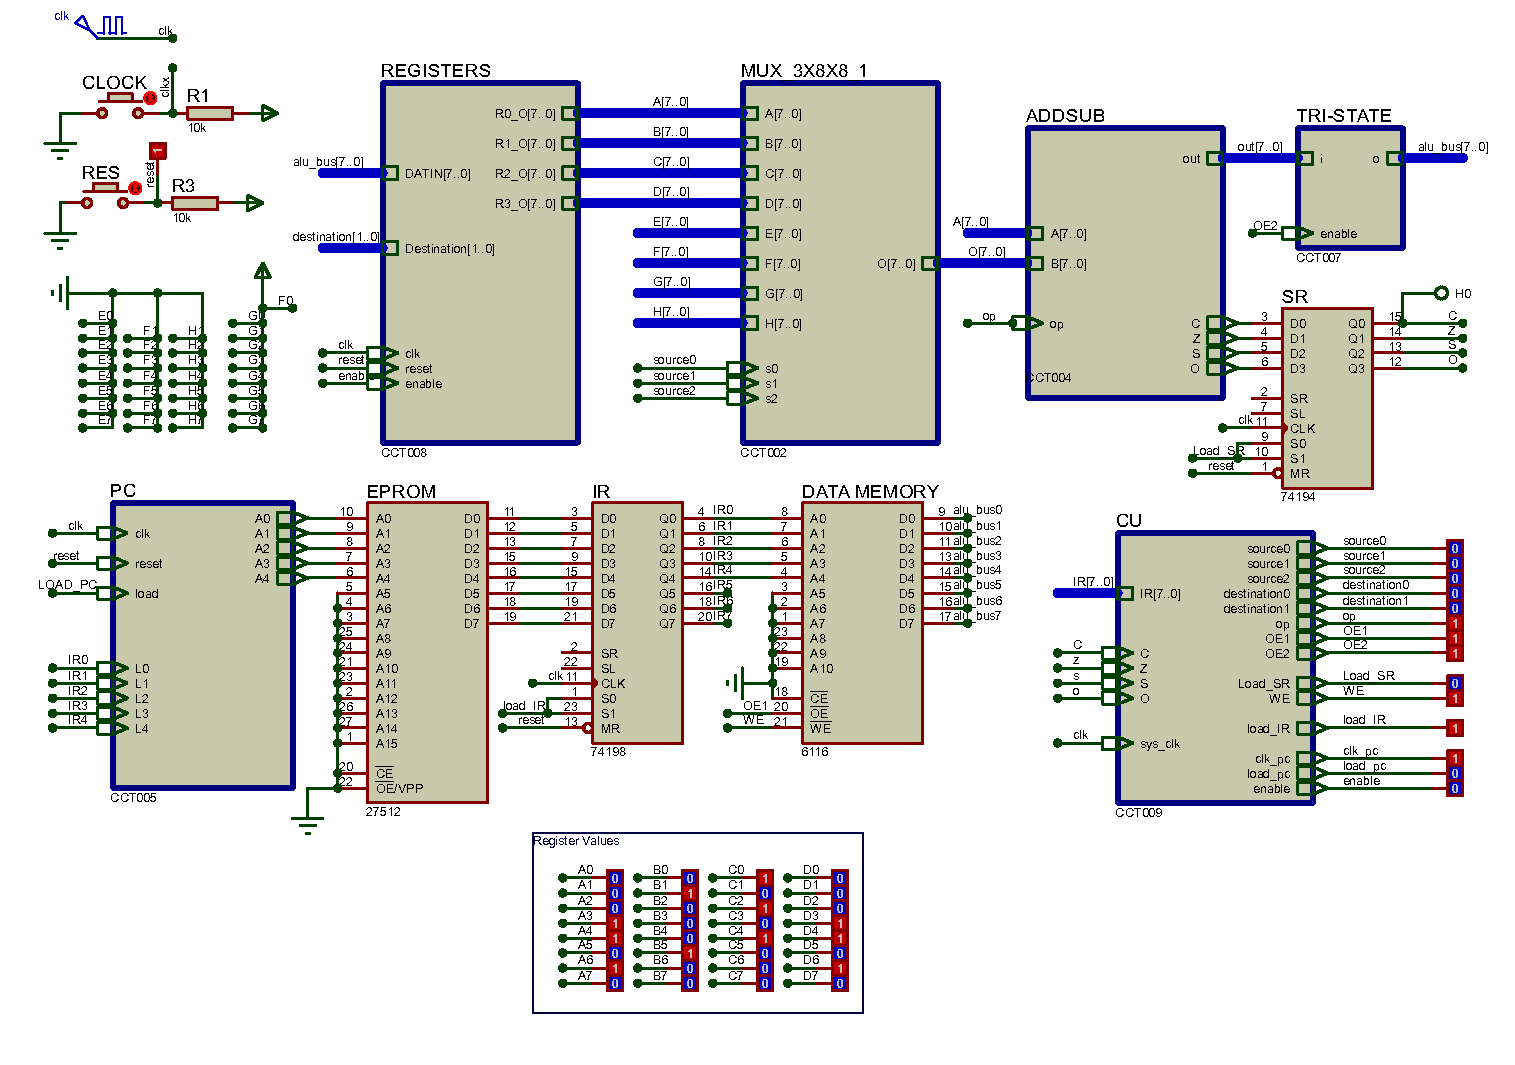
\includegraphics[scale=0.5,page=1]{./graphics/test1}
	\caption{تست اول}
	\label{fig:test1}
\end{figure}
\subsection{جمع دو عدد ۱۶ بیتی}
در دستور کار آزمایش گفته شده بود که دو عدد ۶۴ بیتی از حافظه خوانده و باهم جمع زده شوند ولی به خاطر اینکه نه دستور دسترسی به حافظه غیر مستقیم وجود داشت و نه دستور پرشی مبتنی بر بیت انتقالی و همینطور محدود بودن برنامه ها به ۳۲ دستور متاسفانه گروه ما نتوانست برنامه‌ای بنویسد که خواسته‌های سوال را براورده کند به همین دلیل از یک برنامه برای جمع زدن دو عدد ۱۶ بیتی برای تست کمک گرفته شده است. در ابتدای برنامه اعدادی برای تست درون حافظه ریخته می‌شوند و سپس مراحل جمع آغاز می‌شود در نهایت ۱۶ بیت ریخته شده در حافظه از آن خوانده شده و در ثبات‌های ۰ و ۱ نگه‌داری می‌شوند تا نتیجه مشهود باشد.

برنامه به شکل زیر است:
\begin{latin}
\begin{lstlisting}
			sub		R0,R0	00100000 -> 20
			add		R0,-1	00000110 -> 06     -1
			store   0		01100000 -> 60
			sub		R0,R0   00100000 -> 20
			add		R0,1	00000101 -> 05     1
			add		R0,R0	00000000 -> 00     2
			add		R0,R0	00000000 -> 00     4
			store	1		01100001 -> 61
			add		R0,R0	00000000 -> 00	   8
			store	8		01101000 -> 68
			add		R0,R0   00000000 -> 00     16
			store	9 		01101001 -> 69
			load	0	        01000000 -> 40
			add		R1,0    00001100 -> 0C
			load	8      	    01001000 -> 48
			add		R0,R1	00000001 -> 01
			store	16		01110000 -> 70
			load	1		01000001 -> 41
			add		R0,C	00000111 -> 07
			add		R1,0	00001100 -> 0C
			load	9		01001001 -> 49
			add		R0,R1	00000001 -> 01
			store	17		01110001 -> 71
			add		R1,0	00001100 -> 0C
			load	16		01010000 -> 50
		FAQ:jmp		FAQ		11111001 -> F9
		
		00000100 11111111
		00010000 00001000
		-----------------
		00010101 00000111
\end{lstlisting}
\end{latin}

که در پایان آن ساختار حافظه در نهایت برنامه آمده است. شکل اجرای برنامه در شکل  \ref{fig:test2} آمده است.

\begin{figure}
	\centering
	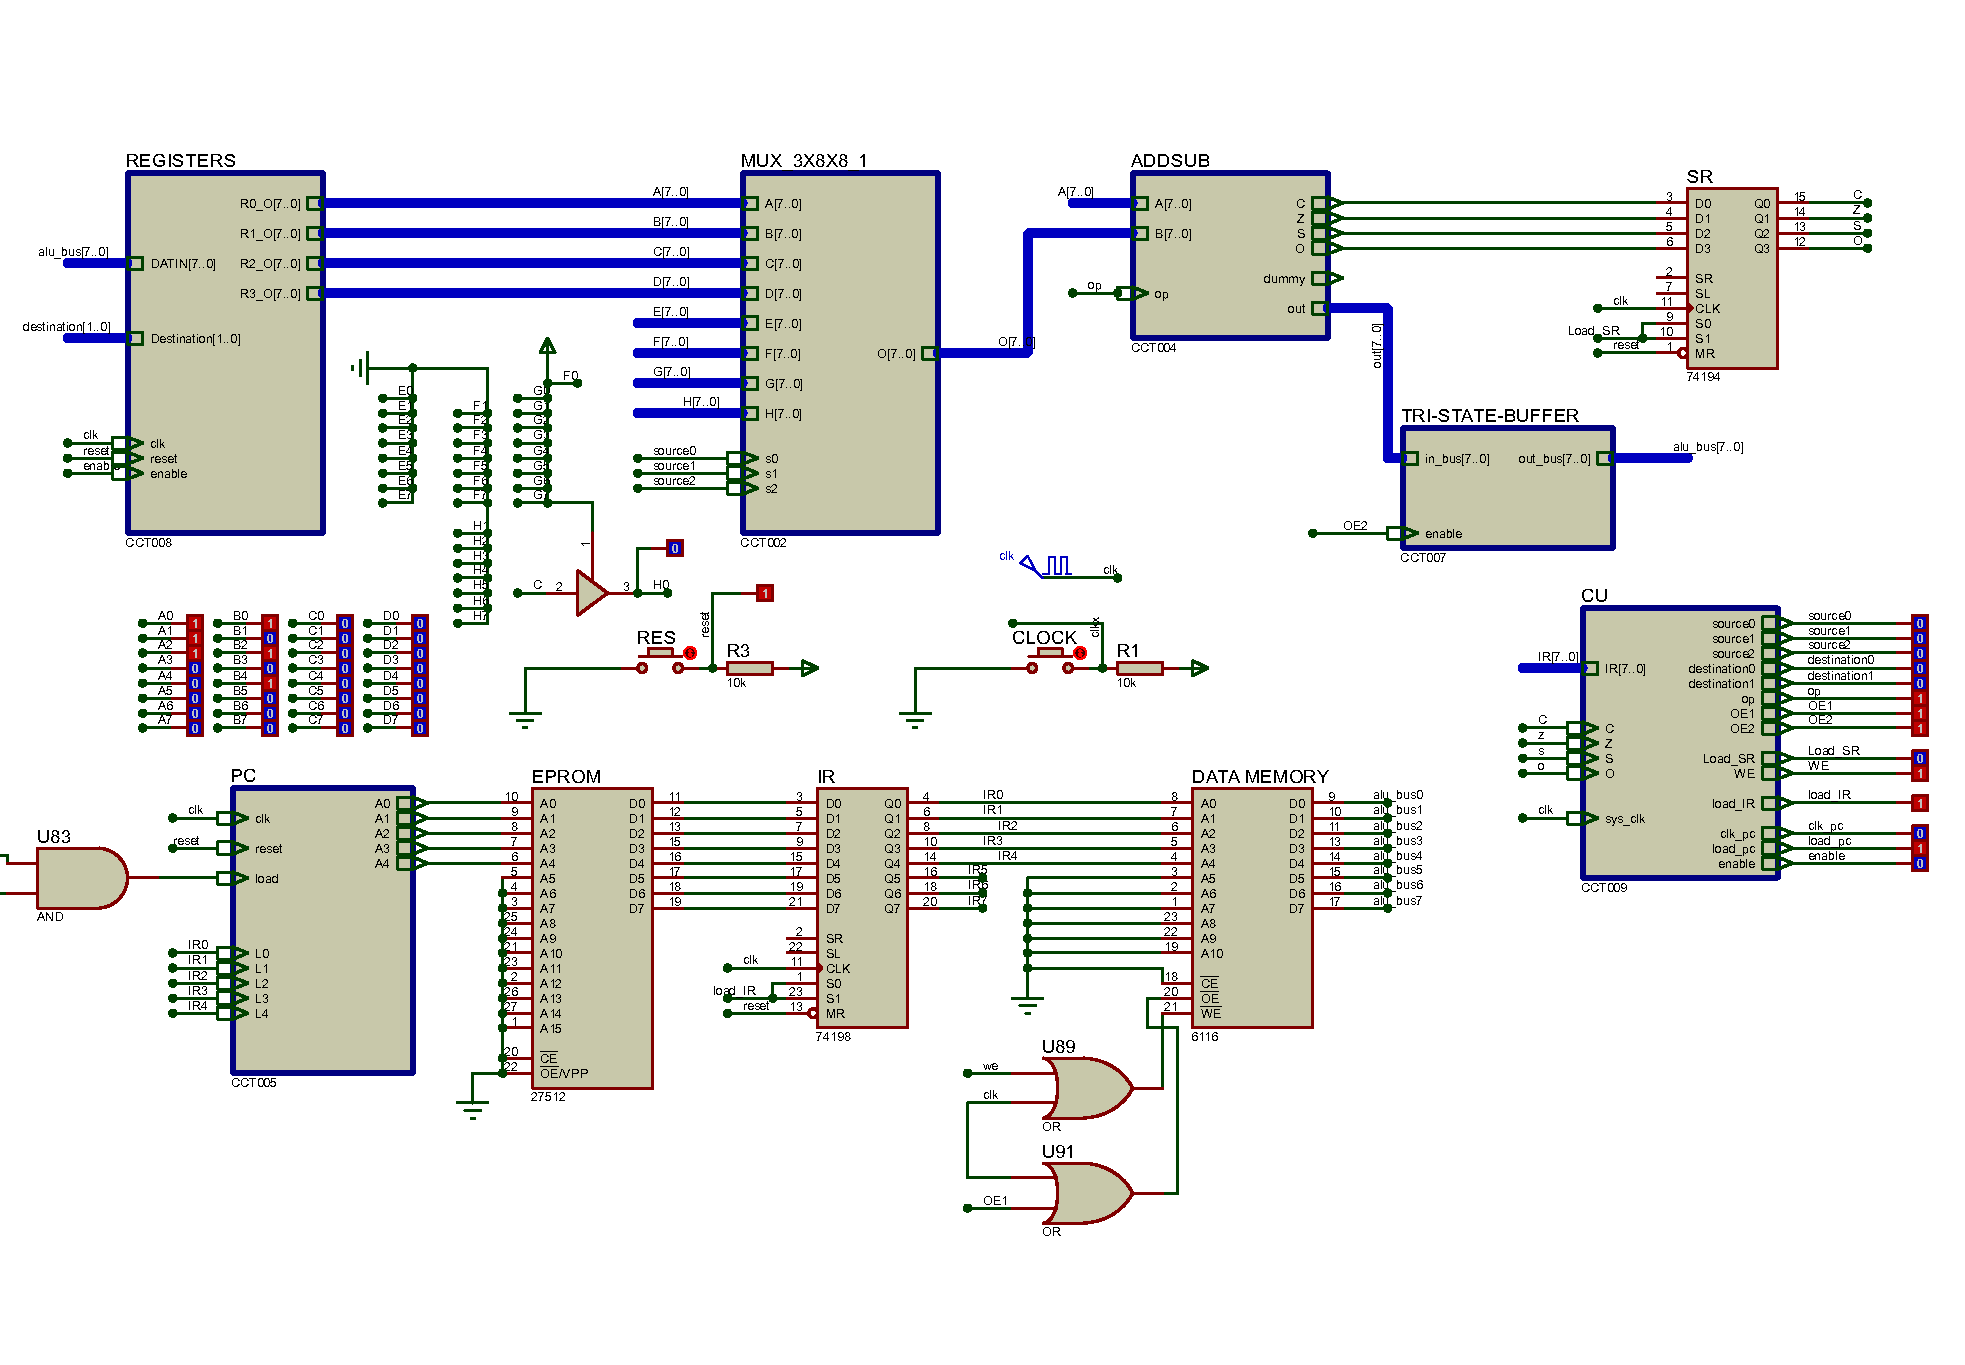
\includegraphics[scale=0.4,page=1]{./graphics/test2}
	\caption{تست دوم}
	\label{fig:test2}
\end{figure}
\end{document}
